\documentclass[12pt,]{article}
\usepackage{lmodern}
\usepackage{amssymb,amsmath}
\usepackage{ifxetex,ifluatex}
\usepackage{fixltx2e} % provides \textsubscript
\ifnum 0\ifxetex 1\fi\ifluatex 1\fi=0 % if pdftex
  \usepackage[T1]{fontenc}
  \usepackage[utf8]{inputenc}
\else % if luatex or xelatex
  \ifxetex
    \usepackage{mathspec}
  \else
    \usepackage{fontspec}
  \fi
  \defaultfontfeatures{Ligatures=TeX,Scale=MatchLowercase}
    \setmainfont[]{Times New Roman}
\fi
% use upquote if available, for straight quotes in verbatim environments
\IfFileExists{upquote.sty}{\usepackage{upquote}}{}
% use microtype if available
\IfFileExists{microtype.sty}{%
\usepackage{microtype}
\UseMicrotypeSet[protrusion]{basicmath} % disable protrusion for tt fonts
}{}
\usepackage[margin=2.54cm]{geometry}
\usepackage{hyperref}
\hypersetup{unicode=true,
            pdftitle={Impacts of Land Use on Water Quality in Minnesota},
            pdfauthor={Keith Bollt, Jake Greif, Felipe Raby-Amadori, \& Lindsay Roth},
            pdfborder={0 0 0},
            breaklinks=true}
\urlstyle{same}  % don't use monospace font for urls
\usepackage{longtable,booktabs}
\usepackage{graphicx,grffile}
\makeatletter
\def\maxwidth{\ifdim\Gin@nat@width>\linewidth\linewidth\else\Gin@nat@width\fi}
\def\maxheight{\ifdim\Gin@nat@height>\textheight\textheight\else\Gin@nat@height\fi}
\makeatother
% Scale images if necessary, so that they will not overflow the page
% margins by default, and it is still possible to overwrite the defaults
% using explicit options in \includegraphics[width, height, ...]{}
\setkeys{Gin}{width=\maxwidth,height=\maxheight,keepaspectratio}
\IfFileExists{parskip.sty}{%
\usepackage{parskip}
}{% else
\setlength{\parindent}{0pt}
\setlength{\parskip}{6pt plus 2pt minus 1pt}
}
\setlength{\emergencystretch}{3em}  % prevent overfull lines
\providecommand{\tightlist}{%
  \setlength{\itemsep}{0pt}\setlength{\parskip}{0pt}}
\setcounter{secnumdepth}{5}
% Redefines (sub)paragraphs to behave more like sections
\ifx\paragraph\undefined\else
\let\oldparagraph\paragraph
\renewcommand{\paragraph}[1]{\oldparagraph{#1}\mbox{}}
\fi
\ifx\subparagraph\undefined\else
\let\oldsubparagraph\subparagraph
\renewcommand{\subparagraph}[1]{\oldsubparagraph{#1}\mbox{}}
\fi

%%% Use protect on footnotes to avoid problems with footnotes in titles
\let\rmarkdownfootnote\footnote%
\def\footnote{\protect\rmarkdownfootnote}

%%% Change title format to be more compact
\usepackage{titling}

% Create subtitle command for use in maketitle
\providecommand{\subtitle}[1]{
  \posttitle{
    \begin{center}\large#1\end{center}
    }
}

\setlength{\droptitle}{-2em}

  \title{Impacts of Land Use on Water Quality in Minnesota}
    \pretitle{\vspace{\droptitle}\centering\huge}
  \posttitle{\par}
  \subtitle{\url{https://github.com/lhr12/HDA_Project}}
  \author{Keith Bollt, Jake Greif, Felipe Raby-Amadori, \& Lindsay Roth}
    \preauthor{\centering\large\emph}
  \postauthor{\par}
    \date{}
    \predate{}\postdate{}
  

\begin{document}
\maketitle

\newpage
\tableofcontents 
\newpage
\listoftables 
\newpage
\listoffigures 
\newpage

\hypertarget{rationale-and-research-questions}{%
\section{Rationale and Research
Questions}\label{rationale-and-research-questions}}

Land use has a large impact on nutrient runoff into streams, lakes, and
other water bodies. Understanding the causes of nutrient problems will
better inform management strategies. A study looking at land use and
water quality in the Chaohu Basin in China found that forest and
grassland has a statistically significant negative correlation with
water quality, while urbanization has a statistically significant
positive correlation with water quality and farmland has a more complex
relationship (Huang et al., 2013). We applied some of the basic research
questions of the Huang et al.~study to the United States. In the US,
nutrient management has been a challenge for states trying to control
harmful algal blooms and coastal dead zones in water bodies like the
Gulf of Mexico (Wurtsbaugh et al., 2019).

We selected the state of Minnesota for our study because it has wide
variety of land uses including a large urban center (the Twin Cities
metropolitan area), natural lands in the northern part of the state, and
large agricultural areas. It also has a large number of lakes with water
quality sampling. Prior studies have shown that water quality in
Minnesota has been adversely affected by land use changes (Christensen
et al., 2012); (Maalim et al., 2013). We also want to look for seasonal
relationships between water quality and land use. For example, we know
that farmers apply nutrients at certain times of year and lakes
naturally have higher levels of algae in summer months.

It is important that states like Minnesota have sound nutrient
management regimes because they affect water quality downstream of their
borders. The Gulf of Mexico has been experiencing hypoxia, or low
dissolved oxygen levels, as a result of agricultural runoff in the
Mississippi River basin. Minnesota is the source of the Mississippi
River and a large agricultural state, so it is important that Minnesota
properly manages its agricultural runoff (Minnesota Pollution Control
Agency, 2019). Our project hopes to make management recommendations for
Minnesota based off our findings.

In order to evaluate the relationship between land use wand lacustrine
water quality in the state of Minnesota, we asked the following two
questions to help guide our research:

\begin{itemize}
\item
  \begin{enumerate}
  \def\labelenumi{\arabic{enumi}.}
  \tightlist
  \item
    What are the predictors of nutrients based on land use in watersheds
    in the state of Minnesota?
  \end{enumerate}

  \begin{itemize}
  \tightlist
  \item
    Hypothesis 1a: The percentage of urbanized land in a lake's
    watershed in the state of Minnesota will have a statistically
    significant negative effect on water quality, as measured by higher
    chlorophyll a concentrations and lower secchi depth measurements.
  \item
    Hypothesis 1b: The percentage of agricultural land in a lake's
    watershed in the state of Minnesota will have a statistically
    significant negative effect on water quality, as measured by higher
    chlorophyll a concentrations and lower secchi depth measurements.
  \item
    Hypothesis 1c: The precentage of undeveloped land in a lake's
    watershed in the state of Minnesota will have a statistically
    significant positive effect on water quality, as measured by lower
    chlorophyll a concentrations and higher secchi depth measurements.
  \end{itemize}
\item
  \begin{enumerate}
  \def\labelenumi{\arabic{enumi}.}
  \setcounter{enumi}{1}
  \tightlist
  \item
    How do you characterize seasonal variation between the predictors of
    nutrients?
  \end{enumerate}

  \begin{itemize}
  \tightlist
  \item
    Hypothesis 2: The water quality in Minnesota lakes will demonstrate
    a statistically significant seasonal pattern.
  \end{itemize}
\end{itemize}

By testing our hypotheses, we aim to accomplish the following goals:

\begin{itemize}
\item
  \begin{enumerate}
  \def\labelenumi{\arabic{enumi}.}
  \tightlist
  \item
    Determine how land use, watershed size, and ecoregion explain
    variation in nutrient loading indicators.
  \end{enumerate}
\item
  \begin{enumerate}
  \def\labelenumi{\arabic{enumi}.}
  \setcounter{enumi}{1}
  \tightlist
  \item
    Discern whether there a seasonal trends in nutrient loading
    indicators based on land use types, watershed size, and ecoregion.
  \end{enumerate}
\item
  \begin{enumerate}
  \def\labelenumi{\arabic{enumi}.}
  \setcounter{enumi}{2}
  \tightlist
  \item
    Provide insight to inform decisions about nutrient management
    practices based on land use types, watershed size, and ecoregion.
  \end{enumerate}
\end{itemize}

\newpage

\hypertarget{dataset-information}{%
\section{Dataset Information}\label{dataset-information}}

The data used in this analysis include data from the Lake Multi-Scaled
Geospatial and Temporal Database (LAGOSNE) and the EPA ecoregion spatial
datasets.

LAGOSNE is a collection of several data modules that contain information
on lakes in the northern United States. The modules contain data from
thousands of lakes in 17 states in the northeastern and midwestern
United States, from Missouri to Maine. The dataset includes a complete
list of all lakes bigger than 4 hectacres in the 17 state area, and
water quality data on a large number of lakes, spanning every state.

Ecoregions are developed by the US Environmental Protection Agency and
are used by planning managers to understand the type of land use that
occurs in different regions of the United States. There are different
levels of ecoregions. Level I has low resolution, and divides North
America into 15 ecological regions, while Level IV offers fine
ecological resolution for each state. This data was published by the
U.S. EPA Office of Research and Development (ORD) - National Health and
Environmental Effects Research Laboratory (NHEERL). Minnesota contains
parts of three distinct Level II ecoregions, which we selected for our
project. This level of resolution allows us to broadly capture the
natural ecosystem variation in different parts of the state in our
statistical models with sufficient water quality data per ecoregion,
conditions that could not be met with higher resolution ecoregions.

\begin{longtable}[]{@{}llll@{}}
\caption{Data structure, including variables, descriptions, units, and
variable types.}\tabularnewline
\toprule
Column.Name & Description & Units & Variable.Type\tabularnewline
\midrule
\endfirsthead
\toprule
Column.Name & Description & Units & Variable.Type\tabularnewline
\midrule
\endhead
chla & Chlorophyll a & micrograms per liter & Dependent\tabularnewline
secchi & Secchi depth & meters & Dependent\tabularnewline
IntenseUrban.pct & \% med. and high intensity urban & \% &
Independent\tabularnewline
OpenUrban.pct & \% developed & \% & Independent\tabularnewline
Barren.pct & \% areas of bedrock and desert pavement & \% &
Independent\tabularnewline
Forest.pct & \% deciduous & \% & Independent\tabularnewline
GrassShrub.pct & \% areas dominated by shrubs & \% &
Independent\tabularnewline
Wetland.pct & \% wetlands & \% & Independent\tabularnewline
Pasture.pct & \% areas of grasses & \% & Independent\tabularnewline
RowCrop.pct & \% cultivated crops & \% & Independent\tabularnewline
LakeIWS.Ratio & Lake surface area to watershed area ratio & N/A &
Independent\tabularnewline
Season & Early/Prime/Late & N/A & Independent\tabularnewline
Ecoregion & Level II Ecoregions & N/A & Independent\tabularnewline
\bottomrule
\end{longtable}

\newpage

\hypertarget{exploratory-analysis}{%
\section{Exploratory Analysis}\label{exploratory-analysis}}

\hypertarget{overview}{%
\subsection{Overview}\label{overview}}

We came in to our exploratory analysis knowing we wanted to look at how
water quality was affected by varying land use. Our exploratory analysis
had four main goals: selecting a study area, selecting a study period,
selecting what land use classifications (independent variables) and
water quality proxies (dependent variables) to study, and preparing a
dataframe to test our research questions and hypotheses.

\hypertarget{data-compilation}{%
\subsection{Data Compilation}\label{data-compilation}}

Our first step was to load the LAGOSNE data columns we though we would
need and to look at how much data each state in our study contained. We
decided on Minnesota because of its high number of lakes in the LAGOSNE
dataset, and its high land use variation. We observed that the latest
land use classification by USGS was from 2011; the second oldest was
from 2006. Therefore, we limited our study to the period from 2009
through 2014 inclusive, so we did not extrapolate too much from our 2011
land use dataset.

\hypertarget{visualize-temporal-distribution-abundance-of-data}{%
\subsubsection{Visualize Temporal Distribution \& Abundance of
Data}\label{visualize-temporal-distribution-abundance-of-data}}

We filtered out just the variables we wanted for our study and created a
``LAGOS.MN.processed'' dataframe. We decided to use chlorophyll a and
secchi depth as proxies of water quality after we visualized our data
and confirmed that we had enough data on these two variables in
Minnesota between 2009 and 2014 to make claims about land use and water
quality; in fact we had over 19,000 lakes with data. Observe in Figure 1
and Table 2 that secchi depth data in Minnesota is available for a large
number of lakes and for a large portion of the year, with gaps in the
data every winter. Observe in Figure 2 and Table 3 a similar pattern in
data availability for chlorophyll a.

\begin{figure}
\centering
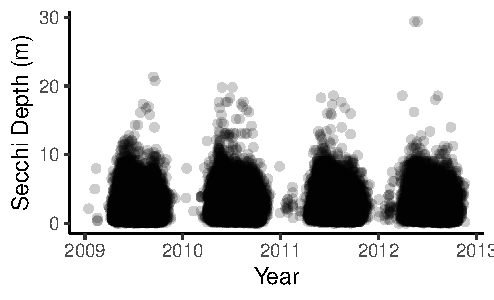
\includegraphics{Bollt_Greif_Raby_Roth_Project_Final_files/figure-latex/Visualize_data-1.pdf}
\caption{This plot provides a sense of how secchi depth measurements are
distributed between and within years, as well as the general range of
secchi depth measurements. Sampling occurs during the middle portion of
each year, and ceases during the winter season.}
\end{figure}

\begin{longtable}[]{@{}lr@{}}
\caption{Number of secchi depth measurements in each of the years to be
included in the analysis, which provides a sense of the amount of data,
as well as the distribution of data.}\tabularnewline
\toprule
Year & Count\tabularnewline
\midrule
\endfirsthead
\toprule
Year & Count\tabularnewline
\midrule
\endhead
2009 & 20849\tabularnewline
2010 & 19829\tabularnewline
2011 & 18025\tabularnewline
2012 & 16924\tabularnewline
\bottomrule
\end{longtable}

\begin{figure}
\centering
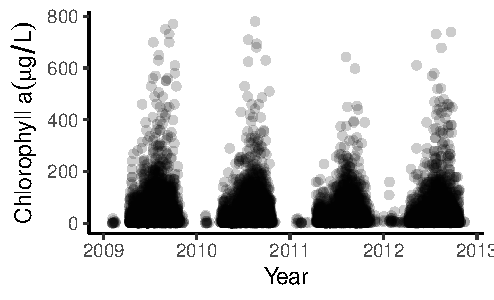
\includegraphics{Bollt_Greif_Raby_Roth_Project_Final_files/figure-latex/unnamed-chunk-3-1.pdf}
\caption{Chlorophyll a vs.~Time. This plot provides a sense of how
chlorophyll a measurements are distributed between and within years, as
well as the general range of chlorophyll a measurements. Sampling occurs
during the middle portion of each year, and ceases during the winter
season.}
\end{figure}

\begin{longtable}[]{@{}lr@{}}
\caption{Number of chlorophyll a measurements in each of the years to be
included in the analysis, which provides a sense of the amount of data,
as well as the distribution of data.}\tabularnewline
\toprule
Year & Count\tabularnewline
\midrule
\endfirsthead
\toprule
Year & Count\tabularnewline
\midrule
\endhead
2009 & 8996\tabularnewline
2010 & 7576\tabularnewline
2011 & 6989\tabularnewline
2012 & 6206\tabularnewline
\bottomrule
\end{longtable}

\hypertarget{explore-trends-in-variables-by-land-use-season}{%
\subsection{Explore Trends in Variables by Land Use \&
Season}\label{explore-trends-in-variables-by-land-use-season}}

We decided what land uses we cared about, based on our background
readings and prior knowledge of water quality and land use, grouped some
land uses together, and assigned them names in our dataframe. We also
created an IWS ratio column, which is the lake area divided by watershed
area. We reasoned a big lake in a small watershed would be affected by
land use differently than a small lake in a big watershed, and we wanted
this to be captured in our analysis.

Our next step was to create a growing ``seasons'' column in order to
account for seasonality in our statistical models. We divided up the
calendar year into three bins: Early (May 15 and Before), Prime (May 16
- September 30), and Late (October 1 and later). These season
designations are somewhat arbitrary, but are based off of our prior
knowledge of when the prime biological growing season is in Minnesota.
We created a dataframe for each of the three seasons.

\hypertarget{visualize-trends-in-variables-by-land-use}{%
\subsubsection{Visualize Trends in Variables by Land
Use}\label{visualize-trends-in-variables-by-land-use}}

Next, we visualized land use percentage versus secchi depth and versus
chlorophyll a for eight representative land uses for the Late season. We
aimed to visually confirm that we might find a relationship between land
use and our two response variables when we ran our statistical tests in
our analysis section. Specifically, we expected to see an increase in
secchi depth and a decrease in chlorophyll a with an increasing
percentage of undeveloped land. Figures 3 and 4 explore the trends in
secchi depth and chlorophyll a by the percentage of each land use type
in the late season. The late season was chosen for exploration because
it had to lowest and highest mean secchi depth and mean chlorophyll a,
respectively. Observe in Figure 3 (secchi depth) and Figure 4
(chlorophyll a) that some ggplots showed a possible relationship between
some land uses and our response variables in the directions that we
predicted in Hypotheses 1a, 1b, and 1c, whereas some ggplots did not
appear to show a relationship.

\begin{figure}
\centering
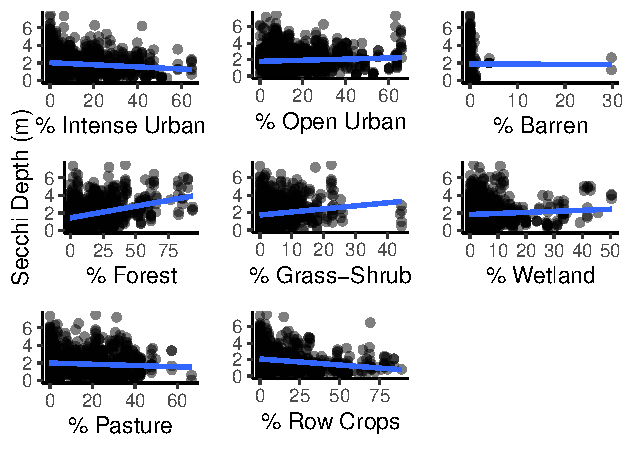
\includegraphics{Bollt_Greif_Raby_Roth_Project_Final_files/figure-latex/unnamed-chunk-6-1.pdf}
\caption{Plots displaying trends in secchi depth relative to the given
land uses during the `Late Season'. The presence of trends supports the
inclusion of the above land uses in the analysis. Note that the x-axes
are on different scales.}
\end{figure}

\begin{figure}
\centering
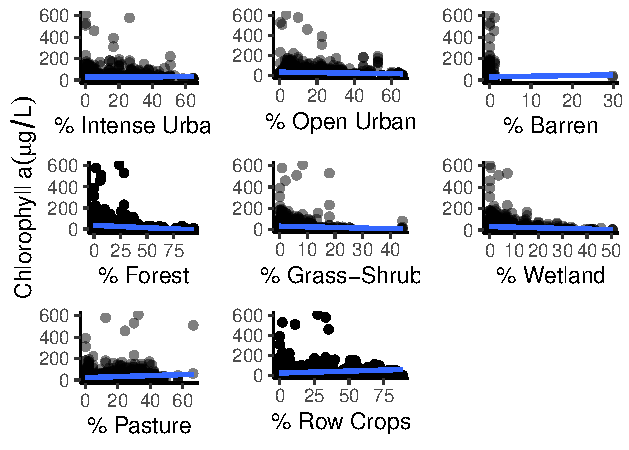
\includegraphics{Bollt_Greif_Raby_Roth_Project_Final_files/figure-latex/unnamed-chunk-8-1.pdf}
\caption{Plots displaying trends in chlorophyll a concentrations
relative to the given land uses during the `Late Season'. The presence
of trends supports the inclusion of the above land uses in the analysis.
Note that the x-axes are on different scales.}
\end{figure}

Because of the presence of some relationships in Figures 3 and 4, we
determined that we had, in fact selected useful land use classifications
and useful seasonal demarcations. We performed a summary function, and
gave all of our columns useful names and removed NAs. Our statistical
tests would not all run if our dataset contained NAs.The next step we
performed was to convert our dataframes to sf dataframes so we could add
Level II ecoregion column.

\hypertarget{visualize-spatial-distribution-of-data-in-each-season}{%
\subsubsection{Visualize Spatial Distribution of Data in Each
Season}\label{visualize-spatial-distribution-of-data-in-each-season}}

Our final exploratory analysis test was to see if we had enough lake
data for each Level II ecoregion for each of our three seasons. We
created three tables, one for each season, with a lake sample count for
each ecoregion. See Tables 4, 5, and 6. From these tables, we learned
that we had enough data to proceed with our statistical analysis, and
therefore Level II ecoregions were the correct resolution for our study.
We also displayed this information spatially in Figures 5, 6, and 7;
each figure corresponds to a different season. We discovered that there
are a large number of lake samples around the Twin Cities area, and that
there is enough spatial variation in our data to capture the three
different Level II ecoregions for all three of our seasons. We concluded
our data wrangling by exporting our three non-sf season processed
dataframes as csv files to our processed data folder.

\begin{figure}
\centering
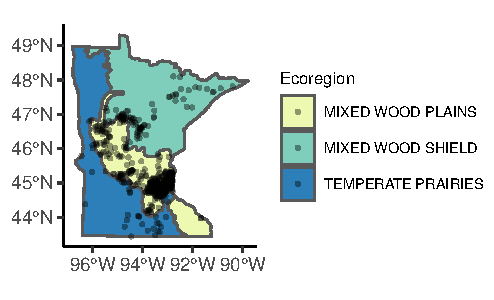
\includegraphics{Bollt_Greif_Raby_Roth_Project_Final_files/figure-latex/unnamed-chunk-10-1.pdf}
\caption{Visual representation of the available secchi depth and/or
chlorophyll a data in each Ecoregion during the `Early Season', which
confirms that there are a suitable number of lakes in each Ecoregion.}
\end{figure}

\begin{longtable}[]{@{}lr@{}}
\caption{Number of lakes with available secchi depth and/or chlorophyll
a data in each Ecoregion during the `Early Season.'}\tabularnewline
\toprule
Ecoregion & Count\tabularnewline
\midrule
\endfirsthead
\toprule
Ecoregion & Count\tabularnewline
\midrule
\endhead
MIXED WOOD PLAINS & 454\tabularnewline
MIXED WOOD SHIELD & 82\tabularnewline
TEMPERATE PRAIRIES & 37\tabularnewline
\bottomrule
\end{longtable}

\begin{figure}
\centering
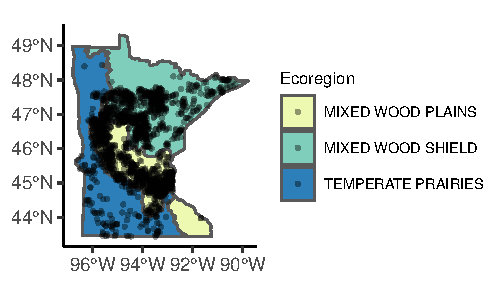
\includegraphics{Bollt_Greif_Raby_Roth_Project_Final_files/figure-latex/unnamed-chunk-12-1.pdf}
\caption{Visual representation of the available secchi depth and/or
chlorophyll a data in each Ecoregion during the `Prime Season', which
confirms that there are a suitable number of lakes in each Ecoregion.}
\end{figure}

\begin{longtable}[]{@{}lr@{}}
\caption{Number of lakes with available secchi depth and/or chlorophyll
a data in each Ecoregion during the `Prime Season.'}\tabularnewline
\toprule
Ecoregion & Count\tabularnewline
\midrule
\endfirsthead
\toprule
Ecoregion & Count\tabularnewline
\midrule
\endhead
MIXED WOOD PLAINS & 1055\tabularnewline
MIXED WOOD SHIELD & 860\tabularnewline
TEMPERATE PRAIRIES & 180\tabularnewline
\bottomrule
\end{longtable}

\begin{figure}
\centering
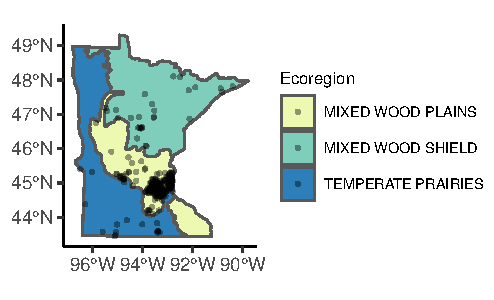
\includegraphics{Bollt_Greif_Raby_Roth_Project_Final_files/figure-latex/unnamed-chunk-14-1.pdf}
\caption{Visual representation of the amount of lakes with available
secchi depth and/or chlorophyll a data in each Ecoregion during the
`Late Season', which confirms that there are a suitable number of lakes
in each Ecoregion.}
\end{figure}

\begin{longtable}[]{@{}lr@{}}
\caption{Number of lakes with available secchi depth and/or chlorophyll
a data in each Ecoregion during the `Late Season.'}\tabularnewline
\toprule
Ecoregion & Count\tabularnewline
\midrule
\endfirsthead
\toprule
Ecoregion & Count\tabularnewline
\midrule
\endhead
MIXED WOOD PLAINS & 278\tabularnewline
MIXED WOOD SHIELD & 28\tabularnewline
TEMPERATE PRAIRIES & 19\tabularnewline
\bottomrule
\end{longtable}

\newpage

\hypertarget{analysis}{%
\section{Analysis}\label{analysis}}

Before creating our models, we tested for autocorrelation between all of
our variables to make sure none of them needed to be excluded. Then, we
tested for normality of the distribution of our variables using qqplots
and Shaprio-Wilkes tests. We used the function BestNormalize to
determine what the best transformation for each variable would be if it
were needed and used that transformation accordingly. We log-transformed
chlorophyll a and secchi depth. We did not find an effective
transformation for our land use variables or the lake IWS ratio, which
we expected because they are proportion and ratio values. Therefore, we
used them in our models with their original distributions.

For our analysis, we ran mixed effect linear models with land use as
fixed effects and ecoregion as random effects in order to account for
variability between ecoregions without considering each ecoregion as its
own factor. We created models for both Chlorophyll a and Secchi depth as
response variables for each of the three seasons making a total of six
models. To determine the most parsimonious models, we eliminated
non-significant variables with the highest p-values one by one until all
remaining variables were significant. To check that this model was the
best fit for the data, we ran an ANOVA on all of the models together to
determine which model had the lowest AIC. If our simplest model had the
lowest AIC or it's AIC was not more than 3 points away from the lowest
score, we chose that model as our best fit.

\hypertarget{question-1}{%
\subsection{Question 1 }\label{question-1}}

\hypertarget{question-2}{%
\subsection{Question 2}\label{question-2}}

\hypertarget{results}{%
\subsection{Results}\label{results}}

Instead of splitting our results into two subsections, one for each
research question, we explore both questions simultaneously. We
formatted our results section in this way because our linear models test
both questions at the same time.

\hypertarget{early-season-chlorophyll-a}{%
\subsubsection{Early Season Chlorophyll
a}\label{early-season-chlorophyll-a}}

The significant predictors of early season chlorophyll a are Open Urban
Percent (p = 2.453 * 10\^{}-5), Forest Percent (p \textless{} 2.2 *
10\^{}-16), Pasture Percent (p = 2.853* 10\^{}-5), Row Crop Percent (p =
0.04671), and Lake IWS Ratio (p = 2.737*10\^{}-6). The marginal R\^{}2 =
0.1058 (represents the variance explained by the fixed effects), and the
conditional R\^{}2 = 0.1058 (interpreted as a variance explained by the
entire model, including both fixed and random effects). Table 7 shows
the coefficients for each significant explanatory variable.

\begin{longtable}[]{@{}lr@{}}
\caption{Model Coefficients. Early Season Chlorophyll a.}\tabularnewline
\toprule
Predictor & Coefficient\tabularnewline
\midrule
\endfirsthead
\toprule
Predictor & Coefficient\tabularnewline
\midrule
\endhead
Open Urban & -0.0107689\tabularnewline
Forest & -0.0152622\tabularnewline
Pasture & 0.0084965\tabularnewline
Row Crop & 0.0032011\tabularnewline
Ratio & -0.3086167\tabularnewline
\bottomrule
\end{longtable}

Since the outcome variable of the model is log transformed, the
coefficients must be exponentiated to be interpreted correctly. In table
8 are presented the percentage increase or decrease that a 1\% increase
of the explanatory variables have on early season chlorophyll a.

\begin{longtable}[]{@{}ll@{}}
\caption{Transformed Model Coefficients. Early Season Chlorophyll
a.}\tabularnewline
\toprule
Predictor & Coefficient\tabularnewline
\midrule
\endfirsthead
\toprule
Predictor & Coefficient\tabularnewline
\midrule
\endhead
OpenUrban & -2.50\%\tabularnewline
Forest & -3.50\%\tabularnewline
Pasture & 2.00\%\tabularnewline
RowCrop & 0.70\%\tabularnewline
LakeIWS.Ratio & -50.90\%\tabularnewline
\bottomrule
\end{longtable}

In figure 8 is shown Early Season log Chlorophyll a vs.~Lake IWS Ratio
together with the Mixed Effects Model that we determined.

\begin{verbatim}
## boundary (singular) fit: see ?isSingular
\end{verbatim}

\begin{figure}
\centering
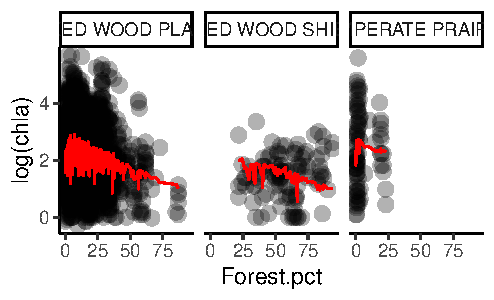
\includegraphics{Bollt_Greif_Raby_Roth_Project_Final_files/figure-latex/unnamed-chunk-19-1.pdf}
\caption{Early Season log Chlorophyll a vs.~Lake IWS Ratio and Mixed
Effects Model}
\end{figure}

\hypertarget{early-season-secchi-depth}{%
\subsubsection{Early Season Secchi
Depth}\label{early-season-secchi-depth}}

The significant predictors of early season secchi depth are Open Urban
Percent (p \textless{} 2.2 * 10\^{}-16), Barren Percent (p = 0.0316103),
Forest Percent (p = \textless{} 2.2 * 10\^{}-16), Grass Shrub Percent (p
= 0.0007119), and Lake IWS Ratio (p = 1.856 * 10\^{}-7). The marginal
R\^{}2 = 0.1081, and the conditional R\^{}2 = 0.2648. This tells us that
16\% of the variability in secchi depth in the early season can be
explained by the variance of ecoregion. Table 9 shows the coefficients
for each significant explanatory variable.

\begin{longtable}[]{@{}lr@{}}
\caption{Model Coefficients. Early Season Secchi Depth.}\tabularnewline
\toprule
Predictor & Coefficient\tabularnewline
\midrule
\endfirsthead
\toprule
Predictor & Coefficient\tabularnewline
\midrule
\endhead
Open Urban & 0.0123681\tabularnewline
Barren & 0.0195641\tabularnewline
Forest & 0.0122881\tabularnewline
Grass Shrub & 0.0102431\tabularnewline
Ratio & 0.2144161\tabularnewline
\bottomrule
\end{longtable}

Since the outcome variable of the model is log transformed, the
coefficients must be exponentiated to be interpreted. In table 10 are
presented the percentage increase or decrease that a 1\% increase of the
explanatory variables have on early season secchi depth.

\begin{longtable}[]{@{}ll@{}}
\caption{Transformed Model Coefficients. Early Season Secchi
Depth.}\tabularnewline
\toprule
Predictor & Coefficient\tabularnewline
\midrule
\endfirsthead
\toprule
Predictor & Coefficient\tabularnewline
\midrule
\endhead
OpenUrban & 2.90\%\tabularnewline
Barren & 4.60\%\tabularnewline
Forest & 2.90\%\tabularnewline
GrassShrub & 2.40\%\tabularnewline
LakeIWS.Ratio & 63.80\%\tabularnewline
\bottomrule
\end{longtable}

In figure 9 is shown Early Season log Secchi Depth vs.~Lake IWS Ratio
together with the Mixed Effects Model that we determined.

\begin{figure}
\centering
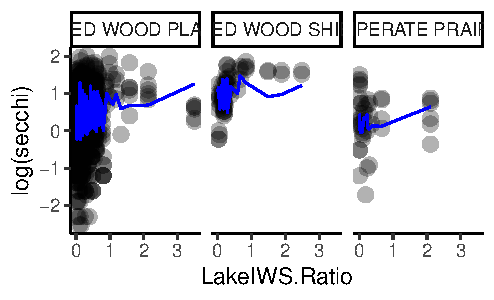
\includegraphics{Bollt_Greif_Raby_Roth_Project_Final_files/figure-latex/unnamed-chunk-22-1.pdf}
\caption{Early Season log Secchi Depth vs.~Lake IWS Ratio and Mixed
Effects Model}
\end{figure}

\hypertarget{prime-season-chlorophyll-a}{%
\subsubsection{Prime Season Chlorophyll
a}\label{prime-season-chlorophyll-a}}

The significant predictors of prime season chlorophyll a are Intense
Urban Percent (p \textless{} 2.2 * 10\^{}-16), Open Urban Percent (p
\textless{} 2.2 * 10\^{}-16), Forest Percent (p \textless{} 2.2 *
10\^{}-16), Grass Shrub Percent (p \textless{} 2.2 * 10\^{}-16), Wetland
Percent (p \textless{} 2.2 * 10\^{}-16), Row Crop Percent (p \textless{}
2.2 * 10\^{}-16), and Lake IWS Ratio (p \textless{} 2.2 *10\^{}-16). The
marginal R\^{}2 = 0.1665 and the conditional R\^{}2 = 0.2513. This tells
us that 9\% of the variability in prime season chlorophyll a can be
explained by the variance of ecoregion. Table 11 shows the coefficients
for each significant explanatory variable.

\begin{longtable}[]{@{}lr@{}}
\caption{Model Coefficients. Prime Season Chlorophyll a.}\tabularnewline
\toprule
Predictor & Coefficient\tabularnewline
\midrule
\endfirsthead
\toprule
Predictor & Coefficient\tabularnewline
\midrule
\endhead
Intense Urban & -0.0100841\tabularnewline
Open Urban & -0.0252362\tabularnewline
Forest & -0.0244790\tabularnewline
Grass Shrub & -0.0252642\tabularnewline
Wetland & -0.0125302\tabularnewline
Row Crop & -0.0069355\tabularnewline
Ratio & -0.4174341\tabularnewline
\bottomrule
\end{longtable}

Since the outcome variable of the model is log transformed, the
coefficients must be exponentiated to be interpreted. In table 12 are
presented the percentage increase or decrease that a 1\% increase of the
explanatory variables have on prime season chlorophyll a.

\begin{longtable}[]{@{}ll@{}}
\caption{Transformed Model Coefficients. Prime Season Chlorophyll
a.}\tabularnewline
\toprule
Predictor & Coefficient\tabularnewline
\midrule
\endfirsthead
\toprule
Predictor & Coefficient\tabularnewline
\midrule
\endhead
IntenseUrban & -2.30\%\tabularnewline
OpenUrban & -5.60\%\tabularnewline
Forest & -5.50\%\tabularnewline
GrassShrub & -5.70\%\tabularnewline
Wetland & -2.80\%\tabularnewline
RowCrop & -1.60\%\tabularnewline
LakeIWS.Ratio & -61.80\%\tabularnewline
\bottomrule
\end{longtable}

In figure 10 is shown Prime Season log Chlorophyll a vs.~Lake IWS Ratio
together with the Mixed Effects Model that we determined.

\begin{figure}
\centering
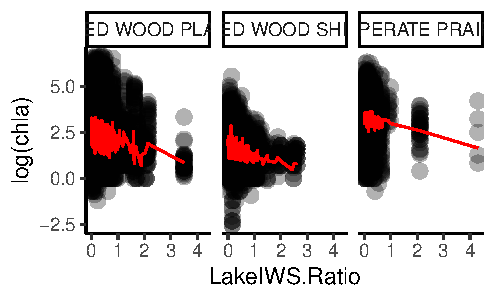
\includegraphics{Bollt_Greif_Raby_Roth_Project_Final_files/figure-latex/unnamed-chunk-25-1.pdf}
\caption{Prime Season log Chlorophyll a vs.~Lake IWS Ratio and Mixed
Effects Model}
\end{figure}

\hypertarget{prime-season-secchi-depth}{%
\subsubsection{Prime Season Secchi
Depth}\label{prime-season-secchi-depth}}

The significant predictors of prime season secchi depth are Intense
Urban Percent (p = 3.028 * 10\^{}-7), Open Urban Percent (p \textless{}
2.2 * 10\^{}-16), Barren Percent (p = 0.04061), Forest Percent (p
\textless{} 2.2 10\^{}-16), Grass Shrub Percent (p \textless{} 2.2 *
10\^{}-16), Pasture Percent (p = 1.234 * 10\^{}-8), Row Crop Percent (p
\textless{} 2.2 * 10\^{}-16), and Lake IWS Ratio (p \textless{} 2.2
*10\^{}-16). The marginal R\^{}2 = 0.1241 and the conditional R\^{}2 =
0.4032. This tells us that 28\% of the variability in prime season
secchi depth can be explained by the variance of ecoregion. Table 13
shows the coefficients for each significant explanatory variable.

\begin{longtable}[]{@{}lr@{}}
\caption{Model Coefficients. Prime Season Secchi Depth.}\tabularnewline
\toprule
Predictor & Coefficient\tabularnewline
\midrule
\endfirsthead
\toprule
Predictor & Coefficient\tabularnewline
\midrule
\endhead
Intense Urban & 0.0042302\tabularnewline
Open Urban & 0.0155867\tabularnewline
Barren & 0.0075966\tabularnewline
Forest & 0.0159693\tabularnewline
Grass Shrub & 0.0144579\tabularnewline
Pasture & 0.0033298\tabularnewline
Row Crop & 0.0046399\tabularnewline
Ratio & 0.3943152\tabularnewline
\bottomrule
\end{longtable}

Since the outcome variable of the model is log transformed, the
coefficients must be exponentiated to be interpreted. In table 14 are
presented the percentage increase or decrease that a 1\% increase of the
explanatory variables have on prime season secchi depth.

\begin{longtable}[]{@{}ll@{}}
\caption{Transformed Model Coefficients. Prime Season Secchi
Depth.}\tabularnewline
\toprule
Predictor & Coefficient\tabularnewline
\midrule
\endfirsthead
\toprule
Predictor & Coefficient\tabularnewline
\midrule
\endhead
IntenseUrban & 1.00\%\tabularnewline
OpenUrban & 3.70\%\tabularnewline
Barren & 1.80\%\tabularnewline
Forest & 3.80\%\tabularnewline
GrassShrub & 3.40\%\tabularnewline
Pasture & 0.80\%\tabularnewline
RowCrop & 1.10\%\tabularnewline
LakeIWS.Ratio & 147.90\%\tabularnewline
\bottomrule
\end{longtable}

In figure 11 is shown Prime Season log Secchi Depth vs.~Lake IWS Ratio
together with the Mixed Effects Model that we determined.

\begin{figure}
\centering
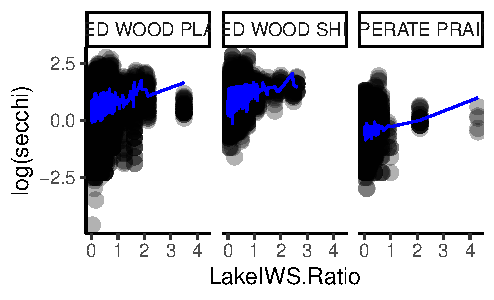
\includegraphics{Bollt_Greif_Raby_Roth_Project_Final_files/figure-latex/unnamed-chunk-28-1.pdf}
\caption{Prime Season log Secchi Depth vs.~Lake IWS Ratio and Mixed
Effects Model}
\end{figure}

\hypertarget{late-season-chlorophyll-a}{%
\subsubsection{Late Season Chlorophyll
a}\label{late-season-chlorophyll-a}}

The significant predictors of late season chlorophyll a are Intense
Urban Percent (p = 3.663* 10\^{}-6), Open Urban Percent (p \textless{}
2.2 * 10\^{}-16), Forest Percent (p \textless{} 2.2 * 10\^{}-16), Grass
Shrub Percent (p = 0.3.231 * 10\^{}-5, coefficient = -0.02814891),
Wetland Percent (p = 0.035393), and Lake IWS Ratio (p = 0.001653). The
marginal R\^{}2 = 0.1515 and the conditional R\^{}2 = 0.2314. This tells
us that 8\% of the variability in late season chlorophyll a can be
explained by the variance of ecoregion. Table 15 shows the coefficients
for each significant explanatory variable.

\begin{longtable}[]{@{}lr@{}}
\caption{Model Coefficients. Late Season Chlorophyll a.}\tabularnewline
\toprule
Predictor & Coefficient\tabularnewline
\midrule
\endfirsthead
\toprule
Predictor & Coefficient\tabularnewline
\midrule
\endhead
Intense Urban & -0.0133056\tabularnewline
Open urban & -0.0237716\tabularnewline
Forest & -0.0248700\tabularnewline
Grass Shrub & -0.0281489\tabularnewline
Wetland & -0.0112842\tabularnewline
Ratio & -0.2633484\tabularnewline
\bottomrule
\end{longtable}

Since the outcome variable of the model is log transformed, the
coefficients must be exponentiated to be interpreted. In table 16 are
presented the percentage increase or decrease that a 1\% increase of the
explanatory variables have on late season chlorophyll a.

\begin{longtable}[]{@{}ll@{}}
\caption{Transformed Model Coefficients. Late Season Chlorophyll
a.}\tabularnewline
\toprule
Predictor & Coefficient\tabularnewline
\midrule
\endfirsthead
\toprule
Predictor & Coefficient\tabularnewline
\midrule
\endhead
IntenseUrban & -3.00\%\tabularnewline
OpenUrban & -5.30\%\tabularnewline
Forest & -5.60\%\tabularnewline
GrassShrub & -6.30\%\tabularnewline
Wetland & -2.60\%\tabularnewline
LakeIWS.Ratio & -45.50\%\tabularnewline
\bottomrule
\end{longtable}

In figure 12 is shown Late Season log Chlorophyll a vs.~Lake IWS Ratio
together with the Mixed Effects Model that we determined.

\begin{figure}
\centering
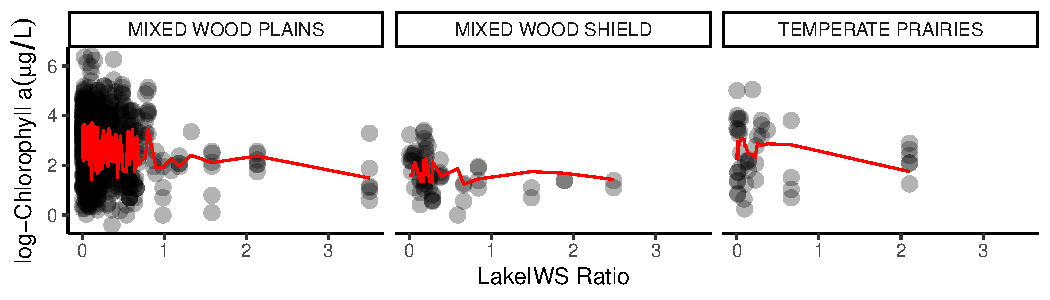
\includegraphics{Bollt_Greif_Raby_Roth_Project_Final_files/figure-latex/unnamed-chunk-31-1.pdf}
\caption{Late Season log Chlorophyll a vs.~Lake IWS Ratio and Mixed
Effects Model}
\end{figure}

\hypertarget{late-season-secchi-depth}{%
\subsubsection{Late Season Secchi
Depth}\label{late-season-secchi-depth}}

The significant predictors of late season chlorophyll a are Intense
Urban Percent (p = 0.03779), Open Urban Percent (p \textless{} 2.2 *
10\^{}-16), Forest Percent (p \textless{} 2.2 * 10\^{}-16), Grass Shrub
Percent (p = 8.468 * 10\^{}-5), and Lake IWS ratio (p = 3.170 *
10\^{}-6). The marginal R\^{}2 = 0.1595 and the conditional R\^{}2 =
0.1889. This tells us that 3\% of the variability in late season secchi
depth can be explained by the variance of ecoregion. Table 17 shows the
coefficients for each significant explanatory variable.

\begin{longtable}[]{@{}lr@{}}
\caption{Model Coefficients. Late Season Secchi Depth.}\tabularnewline
\toprule
Predictor & Coefficient\tabularnewline
\midrule
\endfirsthead
\toprule
Predictor & Coefficient\tabularnewline
\midrule
\endhead
Intense Urban & 0.0038627\tabularnewline
Open Urban & 0.0145363\tabularnewline
Forest & 0.0161930\tabularnewline
Grass Shrub & 0.0176166\tabularnewline
Ratio & 0.2467001\tabularnewline
\bottomrule
\end{longtable}

Since the outcome variable of the model is log transformed, the
coefficients must be exponentiated to be interpreted. In table 18 are
presented the percentage increase or decrease that a 1\% increase of the
explanatory variables have on late season secchi.

\begin{longtable}[]{@{}ll@{}}
\caption{Transformed Model Coefficients. Late Season Secchi
Depth.}\tabularnewline
\toprule
Predictor & Coefficient\tabularnewline
\midrule
\endfirsthead
\toprule
Predictor & Coefficient\tabularnewline
\midrule
\endhead
IntenseUrban & 0.90\%\tabularnewline
OpenUrban & 3.40\%\tabularnewline
Forest & 3.80\%\tabularnewline
GrassShrub & 4.10\%\tabularnewline
LakeIWS.Ratio & 76.50\%\tabularnewline
\bottomrule
\end{longtable}

In figure 13 is shown Late Season log Secchi Depth vs.~Lake IWS Ratio
together with the Mixed Effects Model that we determined.

\begin{figure}
\centering
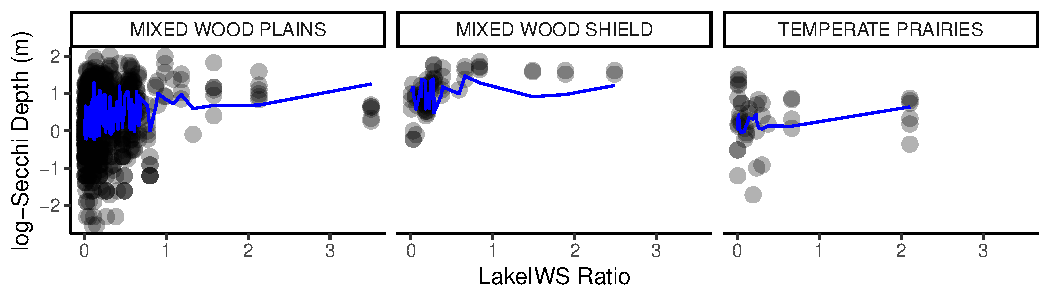
\includegraphics{Bollt_Greif_Raby_Roth_Project_Final_files/figure-latex/unnamed-chunk-34-1.pdf}
\caption{Late Season log Secchi Depth vs.~Lake IWS Ratio and Mixed
Effects Model}
\end{figure}

\newpage

\hypertarget{summary-and-conclusions}{%
\section{Summary and Conclusions}\label{summary-and-conclusions}}

The aim of this project was to examine the impacts that land use had on
water quality in Minnesota and if there was a seasonal characterization
of these effects. Our findings support some of our hypotheses and does
not support others. Our initial assumption as reflected in hypotheses
1a, 1b, and 1c was that urbanized and agricultural land would negatively
impact water quality, and forest and natural lands have positive impact
on water quality. We also predicted in hypothesis 2 that we would see
seasonal variation in our results. Our results are less clear cut than
our hypotheses predicted they would be.

Our second hypothesis is largely supported by our statistical tests. We
found a difference between seasons in our dataset. Observe in Table 7
that no two seasons for the two variables we looked at found the exact
same variance coefficient. In many cases, the difference in coefficients
was quite large, while in other cases the difference was close to
negligible and potentially the result of unaccounted for variation or
statistical noise. Observe our findings for Forest land cover. Prime and
late season have similar results for both chlorophyll a and secchi
depth, but these two values are quite different than the value for early
season. In many cases, we found different significant land uses for the
same dependent variable for different seasons. For example, we found
that Intense Urban only has statistically significant coefficients for
the prime and late seasons. We also found that prime has highest number
of significant variables.

Our first hypothesis is partially supported by our statistical tests.
Observe from Table 7 that our findings do not support our hypotheses 1a,
1b, and 1c for all the land uses that we looked at. Our initial
assumption was that agricultural and urbanized land would negatively
impact water quality, and forest and natural lands would have a positive
impact on water quality. We found that land use has significant impact
on both response variables and that an increase in chlorophyll a was
paired with a decrease in secchi depth in all but one case (row crop,
early). These impacts were sometimes but not always in the direction our
hypotheses predicted.

Row crop showed increasing chlorophyll a in the early season, decreasing
in prime, and was not significant in late. If hypothesis 1b, which dealt
with agricultural land use, was to be true, we would have predicted to
see increasing chlorophyll a for all three seasons. It is worth noting
that the China study by Huang et al. (2013) found a similarly complex
result from agricultural land use. We found several other noteworthy
similarities and differences between our hypotheses 1a, 1b, and 1c:

Similarities to hypotheses:

\begin{itemize}
\tightlist
\item
  Pasture and row crop degrades water quality in early season
\item
  Forest improves water quality all seasons
\item
  Wetland improves water quality prime and late (chlorophyll a only)
\item
  Grass shrub improves water quality
\end{itemize}

Differences from hypotheses:

\begin{itemize}
\tightlist
\item
  Intense urban improves water quality in prime and late season
\item
  Open urban improves in all seasons
\item
  Row crop improves water quality in prime season
\end{itemize}

A major limitation of this study is that it does not consider all of the
factors contributing to water quality. This can be seen in our
relatively low R\^{}2 values for all of our models. Another limitation
is the uneven distribution of lakes across the three ecoregions.
Ecoregions with less lakes will not be as thoroughly accounted for by
this study, and therefore other water quality issues, such as those
related to groundwater, are not captured by this dataset. These
limitations should be considered when developing further studies and
governing policies. Future studies could use more up to date land cover
or alternatively examine the effects of changes in land cover over time.

Our findings offer potential insight for watershed managers in
Minnesota, as well as in the Mississippi River basin. We were able to
show in some cases that increasing the amount of developed land in a
watershed decreases its water quality. In addition, our analysis found
some seasonal variation in water quality. Taken together, these two
findings suggest that land use management decisions in Minnesota
potentially affect water quality far downstream of state lines. We
recommend that managers consider increasing or slowing the decrease of
undeveloped land in Minnesota. Managers also ought to be conscious of
seasonal patterns in water quality impacts of land use. Potentially,
states and Canadian provinces downstream of Minnesota could work
together to improve land use practices at a watershed scale. The
Mississippi River Basin Healthy Watershed Initiative was founded in 2009
and is a 13-state collaborative effort to pool resources from Farm Bill
programs to improve water quality through nutrient management in the
Mississippi River basin (Natural Resources Conservation Service, 2019).
The Initiative is a strong step towards watershed-scale nutrient
management, but it could benefit from an improved understanding of the
types of effects different spatial and temporal land use management
decisions have on downstream water quality.

\newpage

\hypertarget{references}{%
\section{References}\label{references}}

 Christensen, Victoria G., et al. ``Relations between Retired
Agricultural Land, Water Quality, and Aquatic-Community Health,
Minnesota River Basin.'' Journal of Environmental Quality, vol.~41, no.
5, 2012, pp.~1459-72. ProQuest,
\url{https://login.proxy.lib.duke.edu/login?url=https://search.proquest.com/docview/1}
95114913?accountid=10598.

Huang, J., Zhan, J., Yan, H., Wu, F., Xiangzheng Deng, X. ``Evaluation
of the Impacts of Land Use on Water Quality: A Case Study in The Chaohu
Lake Basin,'' The Scientific World Journal, vol.~2013, Article ID
329187, 7 pages, 2013. \url{https://doi.org/10.1155/2013/329187}.

Maalim, Fukhrudin K., Melesse, Assefa M., Belmont, Patrick., Gran, Karen
B. ``Modeling the impact of land use changes on runoff and sediment
yield in the Le Sueur watershed, Minnesota using GeoWEPP.'' CATENA
Volume 107, 2013, Pages 35 45,
\url{https://doi.org/10.1016/j.catena.2013.03.004}.

``Mississippi River Basin Healthy Watersheds Initiative-Natural
Resources Conservation Service.'' Natural Resources Conservation
Service,
\url{https://nrcs.usda.gov/wps/portal/nrcs/detailfull/national/programs/initiatives/?cid=stelprdb1048200}.

``Nutrient Reduction Strategy.'' Minnesota Pollution Control Agency, 6
Mar.~2019,
www.pca.state.mn.us/water/nutrient-reduction-strategy\#resources-b7ca91dc.

Ramstack, Joy M., Sherilyn C. Fritz, and Daniel R. Engstrom. ``Twentieth
Century Water Quality Trends in Minnesota Lakes Compared with
Presettlement Variability.'' Canadian Journal of Fisheries and Aquatic
Sciences, vol.~61, no. 4, 2004, pp.~561-576.


\end{document}
